\documentclass[a4paper]{report}

\usepackage[utf8]{inputenc}

\usepackage{graphicx}
\usepackage{microtype}

% Language & Quotes
% https://de.wikibooks.org/wiki/LaTeX-W%C3%B6rterbuch:_Anf%C3%BChrungszeichen#Anf.C3.BChrungszeichen_mit_dem_Paket_.22csquotes.22
\usepackage[ngerman]{babel}

% font
\usepackage[T1]{fontenc}
\usepackage[sc,osf]{mathpazo}
\linespread{1.05}

% url
% https://de.wikibooks.org/wiki/LaTeX-W%C3%B6rterbuch:_hyperref
\usepackage[pdfborder={0 0 0},colorlinks=true,linkcolor=black,
citecolor=black,filecolor=black,urlcolor=black]{hyperref}

\usepackage{ulem}

% global formating
\pagestyle{headings}
\setcounter{tocdepth}{2}
\setlength{\parindent}{0em}
\setlength{\parskip}{1.0ex plus 1.0ex minus 0.5ex}
\setlength{\labelsep}{1em}

\title{TODO: Name}
\author{Yannic Haupenthal}
\date{30. Januar 2013}

\begin{document}

\pagenumbering{roman}
\pagestyle{empty}

% Titel
\clearpage

% Latex template of:
% http://www.ps-ntf.uni-saarland.de/fileadmin/Benutzerdaten/Downloads/Formulare/Informatik/Abschluss/deckblatt_BA_MA_Dipl_eid_bibo_engl.pdf
% Source: http://www.ps-ntf.uni-saarland.de/index.php?id=80&L=0
\begin{titlepage}

	\vspace*{\fill}

	\begin{center}

	{\large \textbf{Universität des Saarlandes\\
	Naturwissenschaftlich-Technische Fakultät I\\
	Fachrichtung Informatik\\
	Studiengang Medieninformatik}}

	\vspace*{15ex}

	{\large \textbf{Proposal einer Bachelorarbeit}}

	\vspace*{5ex}

	{\Large \textbf{TODO: Name}}

	\vspace*{5ex}

	{\large vorgelegt von

	\textbf{Yannic Haupenthal}

	am 30. Januar 2013
	}

	\vspace*{25ex}

	{\large Angefertigt unter der Leitung von

	Prof.\ Dr.\ Antonio Krüger}

	\vspace*{3ex}
	
	{\large Betreut von

	M.\ Sc.\ Denise Paradowski}

	\end{center}

	\vspace*{\fill}

\end{titlepage}

% Table of contents
\tableofcontents

\clearpage
\pagestyle{headings}

\setcounter{page}{0}
\pagenumbering{arabic}

% Einleitung
\chapter{Einleitung}
\label{chap:introduction}

Als vegan lebender Mensch ist es oft schwer, vegane
Produkte zu finden, wenn nicht schon vorher im Internet recherchiert
wurde. Und selbst dann ist nicht immer direkt ersichtlich warum ein
Produkt unvegan ist (Zutaten sind unbekannt oder haben einen Namen,
der auch tierische Bestandteile beinhalten kann, wie z.\,B. ``Aroma''
oder die
Bakterien der Milchsäuregärung sind tierischer Herkunft oder es
wurde irgendwo im Herstellungsprozess etwas tierisches verwendet, wie
z.\,B. Gelatine bei der Schönung von Wein).

Das alles macht es nicht einfach für den Verbraucher.

Die Idee war daher, eine Webanwendung, bestehend aus Website, mobiler
App und Datenbank, mit
so vielen Produkten wie möglich (und nicht auf Lebensmittel
beschränkt, sondern z.\,B. auch Kosmetika und Textilien) zu erstellen.

Die Datenbank soll entweder genaue Angaben darüber enthalten (durch
Produktanfragen an
den Hersteller), ob das Produkt vegan ist oder nicht\footnote{im
Folgenden als ``Veganität'' bezeichnet}, oder mit Hilfe
schon vorhandener Daten die Wahrscheinlichkeit der Veganität
ermitteln.

Die Website bildet die Grundlage der mobilen App, die zusätzlich noch
einen Barcode Scanner und einen OCR\footnote{Optical Character
Recognition, dt.: Texterkennung}
Reader beinhalten soll.

Alle Bestandteile der Arbeit sollen komplett
als gemeinfreies Werk veröffentlicht werden (auf
Github\footnote{siehe: \url{https://github.com/tohn/bachelor}} und der
Website des
Autors\footnote{siehe: \url{http://yhaupenthal.org/bachelor.htm}}) und
insbesondere auch die
Daten in der Datenbank frei verfügbar sein.

Die Webanwendung wird daher natürlich auch werbefrei und kostenlos
sein.

% Aufgabenstellung
\chapter{Aufgabenstellung}
\label{chap:aufgabenstellung}

Um solch ein Vorhaben zu realisieren, wird eine Datenbank, eine
Website und die mobile App selbst, die wiederum nur aus der mobilen Version
der Website sowie einem Barcode Scanner (und einem OCR Reader)
besteht, benötigt.

Die Datenbank soll Zutaten (z.\,B. E101), Kennzeichen (vegan,
vegetarisch, bio, fair, ...), Benutzer*innen (zum Eintragen), Hersteller,
Produktanfragen, Wahrscheinlichkeiten und die Produkte selbst beinhalten.

Wird ein Produkt mit der mobilen App gescannt, aber nicht in der
Datenbank gefunden, soll es die Möglichkeit geben, das Produkt
direkt mit der App in die Datenbank einzutragen (u.\,a. per Barcode
Scanner und OCR Reader).

Weitere Szenarien sind:

\begin{itemize}
	\item Erstellung einer Produktanfrage, die an den Hersteller
			gesendet werden kann
	\item Angabe von Wahrscheinlichkeiten bzgl. der Veganität (``Für
			wie vegan halten Sie dieses Produkt/diese Zutat'') in Prozent
			$\rightarrow$ daraus können Wahrscheinlichkeiten für
			neue Produkte berechnet werden
	\item Anzeige aller Zutaten auf einen Blick (für den
			Offlinegebrauch); so können einzelne Zutaten auch manuell
			überprüft werden. Dies sähe dann z.\,B. wie auf
			Abbildung~\ref{img:inhaltsstoffe_example} aus.
	\item Änderung bzw. Erweiterung von vorhandenen
			Produkten, Zutaten, Produktanfragen,
			Herstellerinformationen, Kennzeichen und
			Wahrscheinlichkeiten $\rightarrow$ Wikipedia Prinzip (Alle
			angemeldeten Benutzer*innen können alles ändern)
\end{itemize}

\begin{figure}[ht]
	\centering
	\includegraphics{inhaltsstoffe_example-html.png}
	\caption{Drei exemplarische Zutaten; der Farbverlauf kennzeichnet
	die Nutzung für vegan (auf der linken Seite) und vegetarisch (auf
	der rechten Seite) lebende Menschen.}
	\label{img:inhaltsstoffe_example}
\end{figure}

% Loesungsansatz
\chapter{Lösungsansatz}
\label{chap:loesungsansatz}

Wie in der Aufgabenstellung in Kapitel~\ref{chap:aufgabenstellung} beschrieben, braucht es eine
Datenbank, eine Website sowie die darauf basierende mobile App.

\begin{figure}[ht]
	\centerline{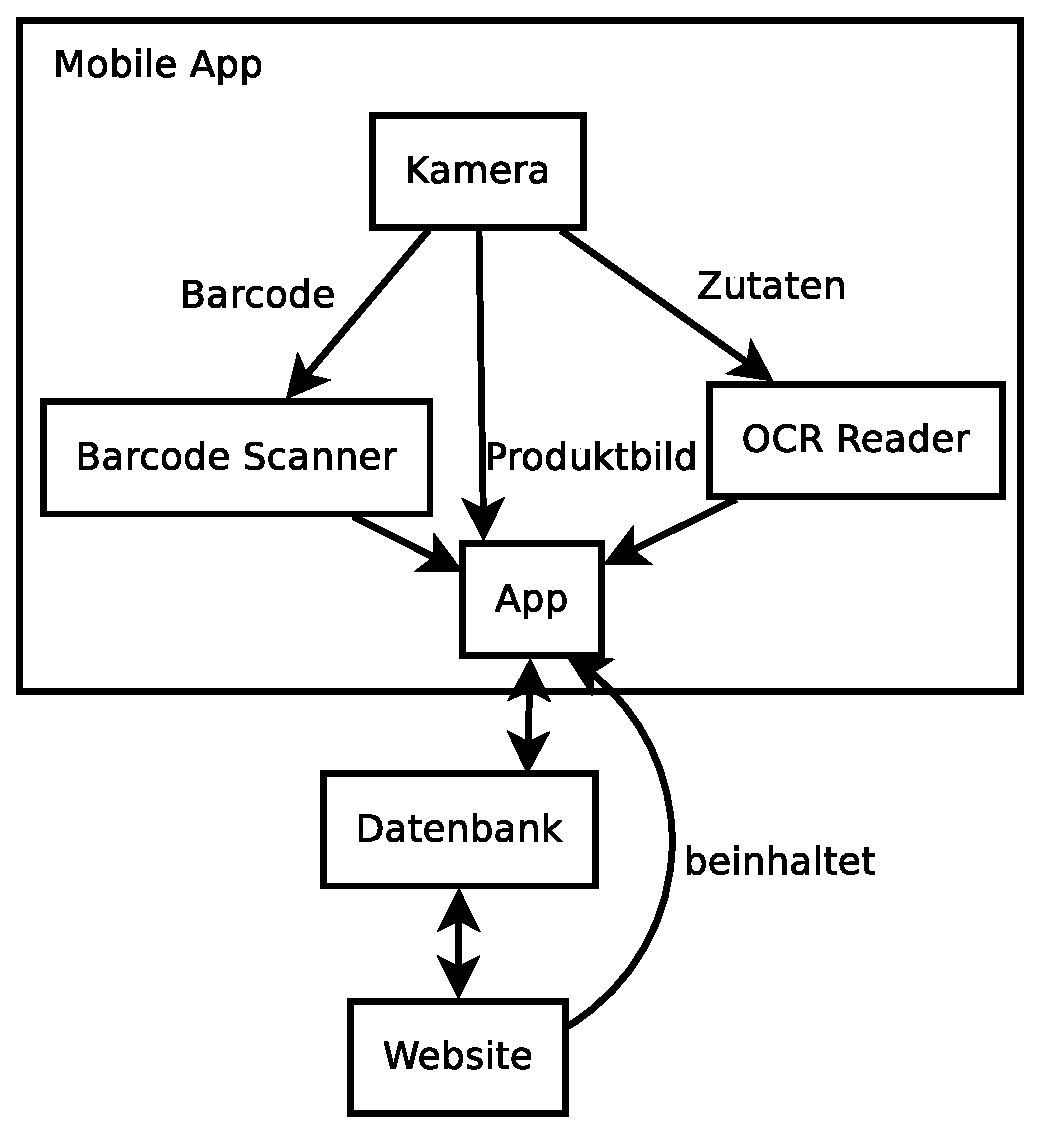
\includegraphics[scale=0.5]{usage_graph.eps}}
	\caption{Die einzelnen Komponenten im Überblick}
	\label{img:usage_graph}
\end{figure}

Wie in Abbildung~\ref{img:usage_graph} gesehen werden kann, spielt die
Datenbank eine große Rolle, denn sie enthält alle Daten, die von der
mobilen App bzw. der Website gebraucht werden.

Die mobile App wiederum benutzt die Kamera um ein Bild von dem Produkt
zu machen, den Barcode auszulesen und wenn möglich, die
Zutaten und weitere Informationen.

Im Folgenden nähere Details zu den drei Hauptkomponenten.

\section{Datenbank}

Die Datenbank (basierend auf
PostgreSQL\footnote{siehe: \url{http://www.postgresql.org/}}) soll 
mehrere Tabellen enthalten:

\subsection{Benutzer*innen}

Zum Anmelden soll OpenID\footnote{siehe: \url{https://openid.net/}} eingesetzt werden.
Unterstüzt werden soll mindestens Google\footnote{siehe:
\url{https://developers.google.com/accounts/docs/OpenID}},
weitere Alternativen (wie Twitter und Facebook) können folgen.

Jedoch müssen einige Informationen (zumindest eine ID, optional noch
Name und Email) in einer Tabelle gespeichert werden. Diese
Informationen werden dann z.\,B. beim automatischen Erstellen einer
Produktanfrage benutzt.

Mit der Speicherung der ID können auch weitere Informationen
gespeichert werden, wie z.\,B. letzte Eintragung eines Produkts,
Produktanfragen von einer/einem Benutzer*in, oder sogar erweiterte Rechte
(keine Überprüfung einer Eintragung mehr notwendig, keine
Überprüfung der eingetragenen Wahrscheinlichkeiten u.\,ä.).

Durch die unterschiedlichen Rechte ergibt sich ein Wikipedia Prinzip,
d.\,h. angemeldete Menschen können alles ändern und Menschen mit
höheren Rechten können anschließend die Änderungen überprüfen.

\subsection{Hersteller}

In dieser Tabelle werden alle Hersteller aufgelistet, dazu auch noch
eine Kontaktadresse (Email). Diese ist sinnvoll für eventuelle
Produktanfragen.

\subsection{Kennzeichen}

Unter Kennzeichen soll alles aufgeführt werden, was ein Produkt bzw.
eine Zutat beschreiben kann.

Dies kann z.\,B. bedeuten, ob ein Produkt eines oder mehrere der 14
Allergene\footnote{siehe:
\url{http://eur-lex.europa.eu/LexUriServ/LexUriServ.do?uri=OJ:L:2007:310:0011:0014:DE:PDF}}
enthält, ob es vegan, vegetarisch, fair, bio, roh,
palmölfrei usw. ist.

\subsection{Produktanfragen}

% Quelle:
% http://www.n-bnn.de/cms/website.php?id=/de/qualitaet/volldeklaration.html
Da die Hersteller in vielen Fällen nicht auf ihr Produkt
schreiben, ob es vegan ist oder nicht und insbesondere nicht einmal
alle Zutaten auflisten (wozu sie nach europäischem Gesetz\footnote{siehe:
\url{http://eur-lex.europa.eu/LexUriServ/LexUriServ.do?uri=OJ:L:2007:310:0011:0014:DE:PDF}}
aber auch nicht gezwungen werden),
ist es für vegan lebende Menschen üblich, direkt beim
Hersteller nachzufragen.

Damit alle Anfragen gespeichert werden und mit dem jeweiligen Produkt
verknüpft werden können, ist diese Tabelle wichtig.

Durch eine Produktanfrage kann eine Wahrscheinlichkeit (die Veganität)
belegt werden.

\subsection{Produkte}

Da in der Datenbank nicht nur Lebensmittel, sondern auch Produkte aus
dem Kosmetik- und Textilbereich, enthalten sein sollen, gibt es
mehrere ``Haupttabellen'' (für jeden Bereich eine), in der alle Informationen
aus den anderen Tabellen zusammenlaufen.

Für jedes Produkt gibt es u.\,a. eine ID, Herstellerangaben, Zeitstempel,
Produktanfragen, Zutaten- und Benutzer*innen-angaben,
Wahrscheinlichkeiten und Produktbilder.

\subsection{Wahrscheinlichkeiten}

Durch Wahrscheinlichkeiten ist es u.\,a. möglich, noch nicht überprüfte
(z.\,B. durch eine Produktanfrage) Produkte bei der Eintragung
automatisch auf Veganität zu prüfen.

Beispiel: Die Zutat ``Aroma'' ist zu 50\,\% vegan, da sich
hinter diesem Namen auch tierische Inhaltsstoffe verstecken können. Alle
anderen deklarierten Zutaten im Produkt sind vegan, d.\,h. das Endprodukt ist nicht
zu 100\,\% vegan und eine Produktanfrage ist nötig.

Ein weiterer Anwendungsfall: Ein Wein wird eingetragen (mit
Wahrscheinlichkeit 100\,\%), aber
Benutzerin xyz hält ihn nicht für vegan, da er womöglich mit
Gelatine geklärt wurde und stuft das Produkt mit 0\,\% auf 50\,\% herab.

\subsection{Zutaten}

Hier sollen alle Zutaten aufgelistet werden. Darunter auch alle
Lebensmittelzusatzstoffe (auch bekannt als E-Nummern).

Um auch Produkte zu speichern, die keine Lebensmittel sind, sollen in
dieser Tabelle auch ``Zutaten'' wie z.\,B. Leder, Wolle, Seide, Pelz und
Daunen sowie Inhaltsstoffe,
wie sie im Kosmetikbereich benutzt werden, enthalten sein.

\section{mobile App}

% Online
Die mobile App auf Basis der Website soll wie zuvor genannt
u.\,a. einen Barcode Scanner enthalten. Wird damit ein Produkt gescannt, soll die
App direkt bei der Datenbank anfragen, ob ein solcher Barcode
existiert. Existiert dieser, werden dann die Informationen zum
Produkt angezeigt.

Existiert der Barcode noch nicht, soll es mit der App möglich sein,
das Produkt in die Datenbank einzutragen. Dazu müssen noch Produktname,
Herstellername und Zutaten angegeben werden (idealerweise mit
OCR Reader). Dies geschieht als anonyme/r oder angemeldete/r Benutzer*in.
Optional kann direkt auch noch ein Bild von dem Produkt aufgenommen und
gespeichert werden.

% Offline
Wie in Kapitel~\ref{chap:aufgabenstellung} schon beschrieben, soll es
noch alle Inhaltsstoffe offline im Überblick geben, die auch durchsucht
werden können und direkt auf einen Blick ersichtlich machen, ob die
Zutat vegan/vegetarisch ist oder nicht.

\section{Website}
\label{website}

Zur einfachen Umsetzung der Website und Datenbank soll das Ruby-on-Rails
Framework\footnote{siehe: \url{http://rubyonrails.org/}} zum Einsatz
kommen. Verwendet werden sollen HTML5, CSS3 und
JavaScript, um eine leichte Benutzer*innen-Interaktion möglich zu machen.

Mit entsprechender Software (z.\,B. PhoneGap\footnote{siehe:
\url{http://phonegap.com/}}) kann diese in eine native App (mit Möglichkeit der
Hardware Nutzung) umgewandelt werden, die
dann auf allen großen mobilen Betriebssystemen läuft (Android, Bada,
BlackBerry OS, iPhone/iOS, Symbian, WebOS, Windows
Phone)\footnote{siehe: \url{http://phonegap.com/about/feature/}} und z.\,B.
auf die Kamera des Smartphones/Tablet-Computers zugreifen kann.

Sollte sich dieser Ansatz als nicht sinnvoll herausstellen (Plugins
zum Barcode lesen und OCR erweisen sich als untauglich) wird es eine
native App für das Android Betriebssystem geben (geschrieben in Java
mit dem Android SDK\footnote{siehe:
\url{https://developer.android.com/sdk/index.html}}).

\clearpage
\section{Externe Daten}

Einige Daten kommen von externer Seite, da diese schon vorhanden und
einfach einbindbar sind.

\subsection{Vegpool}

Dank Kilian Drei{\ss}ig (von Vegpool\footnote{siehe:
\url{http://vegpool.de/}})
dürfen die Inhaltsstoffe von dessen Onlineangebot\footnote{siehe:
\url{http://www.vegpool.de/inhaltsstoffe/index.html}}
per API Zugriff genutzt werden, die er bereits auf Veganität
untersucht hat.

\subsection{Globus Drive}

Globus Drive\footnote{siehe: \url{http://www.globus-drive.de/}} gestattet die
Einbindung ihrer Produktbilder, allerdings nur für den Demonstrator
im IRL\footnote{\label{irl}Innovative
Retail Laboratory, \url{http://www.innovative-retail.de/}} und nicht für die
spätere Veröffentlichung.

\subsection{Globus: SAP}

Globus verwendet im Moment zwei Warenwirtschaftssysteme: ``Dispos'' und ``SAP''.
Da ``Dispos'' durch ``SAP'' ersetzt werden soll, benutze ich nur
letzteres.
In diesem System sind verschiedene Informationen gespeichert, auf
die zugegriffen werden können. Allerdings auch hier nur für den
Demonstrator im IRL.

% Geplantes Vorgehen
\chapter{Geplantes Vorgehen}
\label{chap:vorgehen}

Hier sind alle Meilensteine aufgelistet, zu der die jeweilige
Tätigkeit erledigt sein sollte.

Den Abschluss bildet die Abgabe der Arbeit beim Prüfungsamt\footnote{siehe:
\url{http://www.ps-ntf.uni-saarland.de/}}.

\begin{itemize}
	\item \sout{18.01.2013: Ausarbeitung des Zeitplans}
	\item 31.01.2013: Ausarbeitung des Proposals
	\item 14.02.2013: Ausarbeitung von ``Einleitung'' und ``Motivation''
	\item 15.03.2013: Ausarbeitung von ``Verwandte Arbeiten'' (inkl. verwandte
	Arbeiten studieren)
	\item 31.03.2013: Konzepterstellung
	\item April 2013: Namensfindung und Vortrag im Rahmen des
	Bachelorseminars\footnote{siehe:
	\url{http://www.dfki.de/iui/bms/}}
	\item 31.05.2013: Implementierung (Datenbank, Website, App) und
	Fertigstellung eines ersten Prototyps (wird zu
	Testzwecken/Feedback veröffentlicht)
	\item 15.06.2013: Ausarbeitung der Implementierungskapitel
	\item 30.06.2013: Überarbeitung der Implementierung (mithilfe des Feedbacks)
	\item 15.07.2013: Ausarbeitung von ``Zusammenfassung'' und
	``Ausblick'' $\rightarrow$ \textit{Betaversion} der schriftlichen Arbeit
	\item 31.07.2013: Fertigstellung der Arbeit
\end{itemize}

\end{document}
